\chapter{Discussion}
\label{sec:discussion}

\begin{German}
    In diesem Kapitel wierden die Resultate kritisch reflektiert. Es wird aufgezeigt, was gut funktioniert hat und wo es Schwierigkeiten gab. Zudem wird auf die Limitationen der Fallstudie eingegangen und es werden Empfehlungen für zukünftige Arbeiten gegeben.
\end{German}

\section{Evaluation}
\begin{German}
    Eine umfassende Evaluation der Fallstudie wurde aus zeitgründen von Beginn aus ausgeschlossen. Eine Ground-Truth-Validierung des Modells hat nicht stattgefunden. Die Evaluation beschränkte sich daher auf folgende drei Aspekte:
\end{German}

\begin{English}
    A comprehensive evaluation of the case study was excluded from the beginning due to time constraints. A ground-truth validation of the model did not take place. Therefore, the evaluation was limited to the following three aspects:
\end{English}

\subsection{PolyFit Analysis}
\begin{German}
    Um das Verhalten von PolyFit zu verstehen, wurde während der Entwicklungsphase eine Analyse durchgeführt. Als unabhängige Grösse wurde die Punktanzahl der Punktwolke variiert. Gemessen wurde die Punktdichte, die Laufzeit sowie die Anzahl der Flächen des generierten Modells (siehe \nameref{app:polyfit}). Diese wurde auf einem Intel Core i7-9700K 3.60~GHz Prozessor mit 32~GB RAM durchgeführt.
    
    Zur Bestimmung der Punktdichte wurde zunächst der durchschnittliche Abstand zu den jeweils vier nächsten Nachbarn pro Punkt berechnet. Anschliessend wurde die mittlere Laufzeit sowie deren Standardabweichung bestimmt, die PolyFit für die Rekonstruktion benötigte. Dafür wurde eine Messreihe mit fünf Messungen durchgeführt. Für die jeweils letzte Messung der Messreihe wurde das generierte Modell untersucht. Es wurde visualisiert und die Anzahl der in die Optimierungsaufgabe eingebrachten Flächen als auch die Anzahl der resultierenden Flächen dokumentiert.

    Die Ergebnisse der Analyse wurde für die mittlere Laufzeit und die Flächenanzahl der Modelle visualisiert (siehe Abb. \ref{fig:polyfit_analysis}). Die mittlere Laufzeit steigt mit zunehmender Punktanzahl superlinear an. Die Varianz der Laufzeit sowie die Anzahl der Modellflächen wachsen mit der Punktanzahl an. Grundsätzlich konnte beobachtet werden, dass eine höhere Punktdichte zu komplexeren Modellen führte. Ab einer Punktanzahl von über 100'000 stieg die Laufzeit auf über eine Minute an während die Modellqualität aufgrund zu komplexer Geometrie wieder abnahm. Bei hohen Punktdichten wurden zudem eine hoher Varianz sowohl in der Laufzeit als auch der Anzahl der rekonstuierten Flächen beobachtet. Die subjektiv besten Ergebnisse bei noch tiefer Varianz konnten bei einer Puktanzahl von 70'000 bis 90'000 Punkten beobachtet werden. Dies entsprach einer Punktdichte von 6 bis 7 cm. Die Ergebnisse liesen sich nicht direkt auf die anderen getesteten Gebäude übertragen und mussten individuell bestimmt werden. Es konnte kein Set an Parameter gefunden werden, das für unterschiedliche Gebäude zu zuverlässig guten Ergebnissen führte.
\end{German}

\begin{English}
    To understand the behavior of PolyFit, an analysis was conducted during the development phase. The independent variable was varied by changing the point count of the point cloud. The measured variables included point density, runtime, and the number of faces in the generated model (see \nameref{app:polyfit}). This analysis was performed on an Intel Core i7-9700K 3.60~GHz processor with 32~GB RAM.

    To determine point density, the average distance to the four nearest neighbors for each point was first calculated. Then, the mean runtime and its standard deviation required by PolyFit for reconstruction were determined. A measurement series with five measurements was conducted for each point count. For the last measurement in each series, the generated model was examined. It was visualized, and both the number of faces introduced into the optimization task and the number of resulting faces were documented.

    The results of the analysis were visualized for mean runtime and face count of the models (see Fig. \ref{fig:polyfit_analysis}). The mean runtime increases superlinearly with increasing point count. The variance in runtime and the number of model faces also increase with point count. Generally, it was observed that a higher point density led to more complex models. Above a point count of approximately 110,000, the runtime exceeded one minute while model quality decreased due to overly complex geometry. At high point densities, a high variance in both runtime and number of reconstructed faces was also observed. The subjectively best results with lower variance could be seen at a point count between 70,000 and 90,000 points, corresponding to a point density of 6 to 7 cm. The results could not be directly transferred to other tested buildings and had to be determined individually. No set of parameters was found that consistently led to good results across different buildings.
\end{English}

\begin{figure}[ht]
\centering
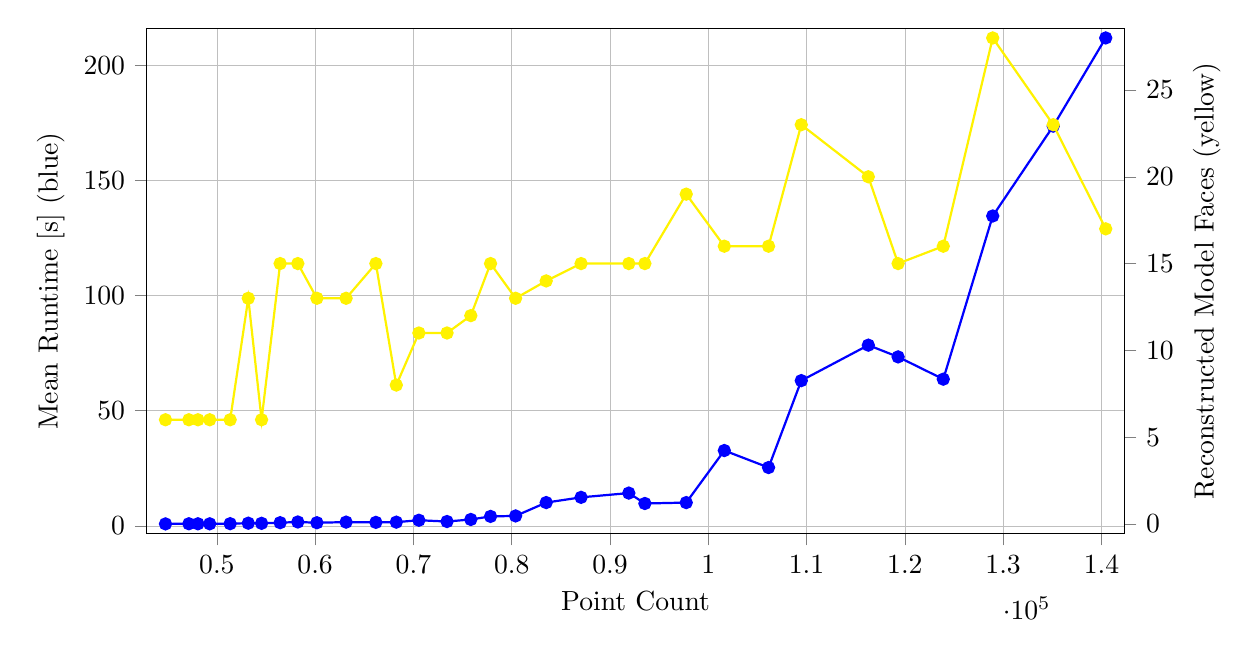
\begin{tikzpicture}
\begin{axis}[
    width=14cm,
    height=8cm,
    xlabel={Point Count},
    ylabel={Mean Runtime [s] (blue)},
    grid=both,
    grid style={line width=.1pt, draw=gray!20},
    major grid style={line width=.2pt,draw=gray!50},
    tick align=outside,
    tick pos=left,
    enlargelimits=0.02,
    legend style={at={(0.5,-0.25)}, anchor=north, legend columns=3},
    ymajorgrids=true,
    xmajorgrids=true,
]

% Erster Plot: mittlere Laufzeit
\addplot[
    color=blue,
    mark=*,
    thick
] coordinates {
    (44774,0.85)
    (47154,0.91)
    (48074,0.90)
    (49276,0.89)
    (51354,0.95)
    (53198,1.16)
    (54552,1.10)
    (56440,1.38)
    (58238,1.68)
    (60179,1.36)
    (63150,1.62)
    (66180,1.51)
    (68259,1.61)
    (70557,2.44)
    (73418,1.88)
    (75839,2.77)
    (77846,4.10)
    (80395,4.31)
    (83509,10.11)
    (87058,12.38)
    (91913,14.23)
    (93549,9.71)
    (97755,10.10)
    (101631,32.70)
    (106131,25.32)
    (109461,63.05)
    (116282,78.45)
    (119312,73.35)
    (123909,63.68)
    (128939,134.52)
    (135094,173.54)
    (140435,211.82)
};
\end{axis}

% Zweite Achse rechts
\begin{axis}[
    width=14cm,
    height=8cm,
    xlabel={},
    ylabel={Reconstructed Model Faces (yellow)},
    axis y line*=right,
    axis x line=none,
    tick align=outside,
    tick pos=right,
    enlargelimits=0.02,
    ymin=0, % <<< Untere Grenze auf 0 setzen
    legend style={at={(0.5,-0.25)}, anchor=north, legend columns=-1},
    ymajorgrids=false,
]

% Zweiter Plot: Anzahl der Flächen
\addplot[
    color=yellow,
    mark=*,
    thick
] coordinates {
    (44774,6)
    (47154,6)
    (48074,6)
    (49276,6)
    (51354,6)
    (53198,13)
    (54552,6)
    (56440,15)
    (58238,15)
    (60179,13)
    (63150,13)
    (66180,15)
    (68259,8)
    (70557,11)
    (73418,11)
    (75839,12)
    (77846,15)
    (80395,13)
    (83509,14)
    (87058,15)
    (91913,15)
    (93549,15)
    (97755,19)
    (101631,16)
    (106131,16)
    (109461,23)
    (116282,20)
    (119312,15)
    (123909,16)
    (128939,28)
    (135094,23)
    (140435,17)
};

\end{axis}
\end{tikzpicture}
\caption{PolyFit Analysis}
\label{fig:polyfit_analysis}
\end{figure}

\subsection{Model Quality}
\begin{German}
    Zur Beurteilung der Modellqualität wurde eine rein qualitative Analyse durchgeführt. Es wurden sowohl die geometrische als auch die semantische Qualität bewertet.
\end{German}

\begin{English}
    To assess the model quality, a purely qualitative analysis was conducted. Both the geometric and semantic quality were evaluated.
\end{English}

\subsubsection{Geometric Quality}
\begin{German}
    Die geometrische Qualität wurde anhand der visuellen Konsistenz der Bauteile beurteilt. Die charakteristische Form des Gebäudes konnte durch das Modell gut wiedergegeben werden. Zu der geometrischen Genauigkeit konnte keine abschliessende Aussage getroffen werden. Das Amt für Baubewilligung hat sich bezüglich den Genauigkeitsanforderungen nicht konkret geäussert. In der Praxis wird als Richtwert eine Genauigkeitstoleranz von 10~cm angestrebt. Ob die Toleranz eingehalten werden konnte, wird angezweifelt. Es konnte eine hohe Variation der generierten Modelle beobachtet werden. Die Reproduzierbarkeit war tief. Selbst bei gleichbleibenden Parametern wurden teilweise unterschiedliche Modelle generiert. Es wird vermutet, dass die tiefe Präzision die Folge des nicht deterministischen RANSAC-Algorithmus oder einer Mehrdeutigkeit des Optimierungsproblems sein könnte. Die tiefen Präzision führt letzlich zu einer tiefen geometrischen Genauigkeit.

    Nebst der geometrischen Genauigkeit ist auch die Vollständigkeit des Modells von Bedeutung. Hier konnte beobachtet werden, dass teilweise als relevant erachtete Bauteile nicht im Modell enthalten waren. So wurde beispielsweise der Schachtkopf nicht modelliert.

    Eine weitere Herausforderung stellten die geometrischen Impferfektionen dar. Es ist anzunehmen, dass die Deckenplatten zueinander geringfügig weniger parallel verlaufen als im realen Bauwerk. Zudem zeigen die Wände eine unsystematische Neigung. Diese Imperfektionen mögen für die Baueingabe vernachlässigbar sein, konnten aber die Bearbeitbarkeit der parametrisierten Bauteile einschränken. Dies erscheint plausibel, da beispielsweise eine geneigte Wand nicht mehr allein durch eine Basislinie und einer dazugehörigen Höhe dargestellt werden kann. Ohne die Bearbeitbarkeit kann das Bauteil geometrisch nicht angepasst werden, was die Verwendung in der Praxis stark einschränken kann.
\end{German}

\begin{English}
    The geometric quality was assessed based on the visual consistency of the components. The characteristic shape of the building was well represented in the model. No conclusive statement could be made regarding geometric accuracy. The Building Permit Office did not specify concrete accuracy requirements. In practice, a guideline accuracy tolerance of 10~cm is aimed for. It is doubted whether this tolerance was met. A high variation of the generated models was observed, and reproducibility was low. Even with consistent parameters, different models were sometimes generated. It is suspected that the low precision may be due to the non-deterministic RANSAC algorithm or an ambiguity in the optimization problem. Ultimately, the low precision leads to low geometric accuracy.

    In addition to geometric accuracy, the completeness of the model is also important. It was observed that some components considered relevant were not included in the model, such as the shaft head.

    Another challenge was geometric imperfections. It is assumed that the slabs are slightly less parallel to each other than in the actual building. Additionally, the walls show an unsystematic inclination. While these imperfections may be negligible for permit purposes, they can limit the usability of parameterized components. This seems plausible since, for example, an inclined wall cannot be represented solely by a base line and a corresponding height. Without usability, the component cannot be geometrically adjusted, which can significantly restrict its practical use.
\end{English}

\subsubsection{Semantic Quality}
\begin{German}
    Die semantische Qualität des Modells wurde anhand der korrekten Klassifizierung der Bauteile bewertet. Eine korrekte Klassifizierung der Bauteile ist besonders für die automatisierte Parametrisierung von Bedeutung. Die 14 Bauteile wurden korrekt klassifiziert, mit Ausnahme einer ungenau rekonstruierten Wand. Die Wand wurde schräg modelliert, wodurch der Normalenvektor eine z-Komponente aufwies und als Dach (\texttt{IfcRoof}) klassifiziert wurde. Die semantische Qualität hängt damit stark von der geometrischen Qualität ab.
\end{German}

\begin{English}
    The semantic quality of the model was assessed based on the correct classification of the components. Correct classification of components is particularly important for automated parameterization. The 14 components were correctly classified, with the exception of one inaccurately reconstructed wall. The wall was modeled at an angle, resulting in a normal vector with a z-component, which led to its classification as a roof (\texttt{IfcRoof}). Thus, the semantic quality is strongly dependent on the geometric quality.
\end{English}

\subsection{Transferability to other buildings}
\begin{German}
    Um die Übertragbarkeit des entwickelten Frameworks auf unterschiedliche Gebäudetypen zu prüfen, wurden exemplarisch vier Gebäude rekonstruiert und die Ergebnisse qualitativ ausgewertet. Modelliert wurden eine Kapelle (1), ein Einfamilienhaus mit Giebeldach (2), ein landwirtschaftlicher Hallenbau (3) sowie ein moderner Wohnkomplex (4). Die Resultate sind in Abbildung~\ref{fig:transferability} dargestellt.

\begin{enumerate}
    \item Das schwächste Ergebnis wurde bei Gebäude 1 erzielt. Die Rekonstruktion des runden Turmaufsatzes führte zu geometrischen Artefakten. Die charakteristische Form des Gebäudes konnte im Modell nur unzureichend wiedergegeben werden.
    \item Die Gebäude 2 bis 4 wurden insgesamt gut rekonstruiert, wobei bei den Modellen 2 und 4 jeweils markante Bauteile durch Generalisierung verloren gingen.
\end{enumerate}

    Insgesamt konnte gezeigt werden, dass das Framework grundsätzlich auf unterschiedliche Gebäudetypen anwendbar ist. Die Ergebnisse deuten darauf hin, dass grossflächige Gebäude mit einfachen Geometrien tendenziell zuverlässiger rekonstruiert werden können.
\end{German}

\begin{figure}[htbp]
        \centering
        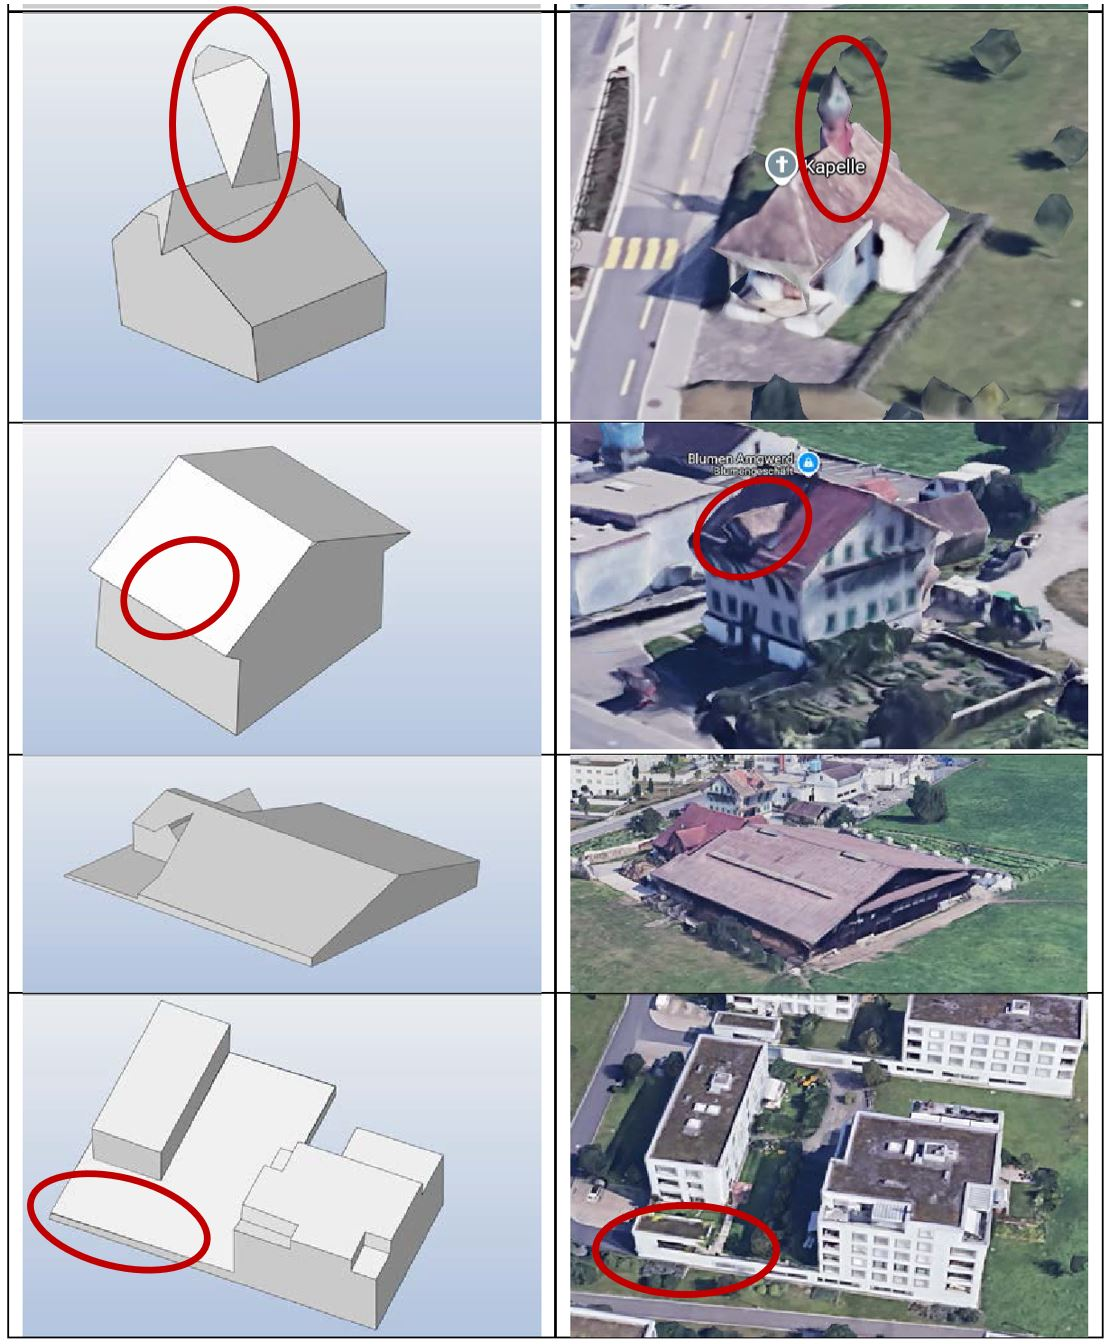
\includegraphics[width=0.8\textwidth]{images/transferability.JPG}
        \caption{Transferability to other building types}
        \label{fig:transferability}
\end{figure}

\begin{English}
    To test the transferability of the developed framework to different building types, four buildings were reconstructed as examples, and the results were qualitatively evaluated. The buildings modeled include a chapel (1), a single-family house with a gable roof (2), an agricultural hall building (3), and a modern residential complex (4). The results are shown in Figure~\ref{fig:transferability}.

    \begin{enumerate}
        \item The weakest result was achieved with building 1. The reconstruction of the round tower top led to geometric artifacts. The characteristic shape of the building could only be inadequately represented in the model.
        \item Buildings 2 to 4 were generally reconstructed well, although in models 2 and 4, significant components were lost due to generalization.
    \end{enumerate}

    Overall, it was shown that the framework is fundamentally applicable to different building types. The results suggest that large-area buildings with simple geometries can be reconstructed more reliably.
\end{English}

\section{Limitations}
\begin{German}
    Das entwickelte Framework weist noch einige Limitationen auf, die die Anwendbarkeit in der Praxis einschränken können. Die Limitationen können aufgrund ihrer Herkunft in drei Kategorien eingeteilt werden.
\end{German}

\begin{English}
    The developed framework still has some limitations that may restrict its applicability in practice. The limitations can be categorized based on their origin.
\end{English}

\subsubsection{Limitations in Geometric Reconstruction}
\begin{German}
    Die grösste Limitierung kann derzeit in Zusammenhang mit der geometrischen Rekonstruktion gebracht werden. Einschränkungen die damit einhergegen sind:

    \begin{itemize}
        \item Das Framework kann nur auf isolierte, einzelne Gebäude angewendet werden.
        \item Das Framework kann nicht zuverlässig auf gekrümmte oder komplexe Geometrien angewendet werden. Was als komplexe Geometrie gilt, konnte nicht abschliessned definiert werden und muss im Einzelfall beurteilt werden.
        \item Das Framework erfüllt die in der Praxis geforderten Genauigkeitsanforderungen von 10~cm wahrscheinlich nicht.
        \item Das Framework hat eine geringe Reproduzierbarkeit. Die Variation der generierten Modelle ist hoch. Es müssen subjektive Entscheidungen getroffen werden, die die Reproduzierbarkeit weiter einschränken.
        \item Das Framework führt zu geometrisch imperfekten Modellen. Die Imperfektionen können die Modellierung erschweren und die Parametrisierung einschränken. 
    \end{itemize}
\end{German}

\begin{English}
    The biggest limitation is currently related to geometric reconstruction. At the same time, it is the most complex part of the framework, contributed by scientific research, and is unlikely to be optimized further. Limitations associated with this are:

    \begin{itemize}
        \item The framework can only be applied to isolated, individual buildings.
        \item The framework cannot be reliably applied to curved or complex geometries. What constitutes a complex geometry could not be conclusively defined and must be assessed on a case-by-case basis.
        \item The framework likely does not meet the accuracy requirements of 10~cm demanded in practice.
        \item The framework has low reproducibility. The variation of generated models is high. Subjective decisions must be made, further limiting reproducibility.
        \item The framework leads to geometrically imperfect models. These imperfections can complicate modeling and restrict parameterization.
    \end{itemize}
\end{English}

\subsubsection{Limitations in Automation}
\begin{German}
    Die Automatisierung des Frameworks ist derzeit noch unvollständig. Es müssen manuelle Anpassungen vorgenommen werden, um ein brauchbares BIM-Modell zu erhalten. Dies führt zu Diese sind:

    \begin{itemize}
        \item Das Framework konnte nicht vollständig automatisiert werden. Es müssen manuelle Anpassungen vorgenommen werden, um ein brauchbares BIM-Modell zu erhalten.
        \item Das Framework kann derzeit ausschliesslich automatisierte IFC-Modelle generieren. Die Generierung von parametrisierten Modellen ist derzeit nicht möglich.
    \end{itemize}
\end{German}

\begin{English}
    The automation of the framework is currently incomplete. Manual adjustments must be made to obtain a usable BIM model. These limitations are:

    \begin{itemize}
        \item The framework could not be fully automated. Manual adjustments are necessary to obtain a usable BIM model.
        \item The framework can currently only generate automated IFC models. The generation of parameterized models is not possible at this time.
    \end{itemize}
\end{English}

\subsubsection{Limitations in Usability and Integration}
\begin{German}
    Das Framework wurde für die Fallstudie entwickelt und nicht für den produktiven Einsatz. Dies führt zu weiteren Limitationen:

    \begin{itemize}
        \item Das Framework lässt sich derzeit nicht effizient depolyen. Abhängigkeiten führen zu erhötem Setupaufwand. Die Installation setzt Grundkentnisse in Python-Tooling voraus.
        \item Das Framework ist nicht intuitiv bedienbar. Es besteht aus mehreren Python-Skripten, in denen bei schlechter Performanz noch Hyperparameter angepasst werden müssen. Eine technische Dokumentation fehlt.
        \item Das Framework setzt Kentnisse in manueller BIM-Modellierung voraus. Ohne entsprechende Kentnisse kann mit dem Framework lediglich ein IFC-Modell generiert werden. 
        \item Das Framework kann derzeit ausschliesslich auf .ply-Punktwolkenformate angewendet werden. Andere Punktwolkenformate werden nicht unterstützt.
    \end{itemize}
\end{German}

\begin{English}
    The framework was developed for the case study and not for productive use, leading to further limitations:

    \begin{itemize}
        \item The framework cannot currently be deployed efficiently. Dependencies lead to increased setup effort. Installation requires basic knowledge of Python tooling.
        \item The framework is not intuitively usable. It consists of several Python scripts, where hyperparameters must still be adjusted in case of poor performance. A technical documentation is missing.
        \item The framework requires knowledge of manual BIM modeling. Without corresponding knowledge, only an IFC model can be generated with the framework.
        \item The framework can currently only be applied to .ply point cloud formats. Other point cloud formats are not supported.
    \end{itemize}
\end{English}

\section{Future Work}
\begin{German}
    Die Limitationen des Frameworks schränken die Anwendbarkeit in der Praxis stark ein. Um das Framework für den produktiven Einsatz zu optimieren, sollten folgende Punkte angegangen werden:
\end{German}

\begin{English}
    The limitations of the framework significantly restrict its applicability in practice. To optimize the framework for productive use, the following points should be addressed:
\end{English}

\subsubsection{Future Work in Geometric Reconstruction}
\begin{German}
    Der Limitierungsbeitrag der geometrischen Rekonstruktion wird insgesamt am höchten eingeschätzt und sollte daher priorisiert angegegangen werden. Gleichzeitig ist es der komplexeste Teil des Frameworks, der aus der Forschung stammt. Die Wahrscheinlichkeit einer Optimierung des eigentlichen Algorithmus wird als unrealistisch eingestuft. Es wird daher empfohlen, alternative Tools für die geometrische Rekonstruktion auszuprobieren. Dank des modularen Aufbaus des Frameworks, können die Tools ausgetauscht werden, ohne Auswirkung auf die anderen Teile zu haben. Methoden die auf Annahmen wie "Manhatten-Assumption" basieren, können hier vielversprechend sein. Diese Annahme führt dazu, dass die Geometrie des Gebäudes auf rechtwinklige Bauteile beschränkt wird. Diese Annahme dürfte auf viele Gebäude zutreffen und dürfte zu sauberen Modellen führen. Als konkrete Handlungsempfehlung wird vorgeschalgen:

    \begin{itemize}
        \item \textbf{Hohe Priorität:} Ersatz von PolyFit durch ein alternatives Tool. \cite{wangReconstructionLoD2Building2023} sieht nach einer ersten Analyse vielversprechend aus. Ob der Quellcode zugänglich ist, muss geprüft werden.
        \item \textbf{Hohe Priorität:} Alternativ wird empfohlen, den Entwockler von PolyFit, Professor Dr. Liangliang Nan von der TU Delft zu kontaktieren. Er zeigte sich bereits bei der Implementierung hilfsbereit und könnte wertvolle Hinweise geben, welche Alternativen in Frage kommen.
    \end{itemize}
\end{German}

\begin{English}
    The contribution of limitations from geometric reconstruction is overall considered the highest and should therefore be prioritized. At the same time, it is the most complex part of the framework, stemming from research. The likelihood of optimizing the actual algorithm is deemed unrealistic. It is therefore recommended to try alternative tools for geometric reconstruction. Thanks to the modular structure of the framework, tools can be replaced without affecting other parts. Methods based on assumptions like the "Manhattan Assumption" can be promising here. This assumption leads to the geometry of the building being limited to right-angled components, which is likely applicable to many buildings and should result in clean models. For future implementations, the following is recommended:

    \begin{itemize}
        \item \textbf{High Priority:} Replace PolyFit with an alternative tool. \cite{wangReconstructionLoD2Building2023} looks promising based on initial analysis, but accessibility of the source code needs to be verified.
        \item \textbf{High Priority:} Alternatively, it is recommended to contact the developer of PolyFit, Professor Dr. Liangliang Nan from TU Delft. He has been helpful during implementation and could provide valuable insights into potential alternatives.
    \end{itemize}
\end{English}

\subsubsection{Future Work in Automation}
\begin{German}
    Die Automatisierung des Frameworks ist derzeit unvollständig. Es wird empfohlen, die Automatisierung weiter voranzutreiben. Als mit wenig Aufwand realisierbar eingestuft wird die automatische Parametrisierung des IFC-Modells mit Dynamo. Eine daraüber hinausgehende, vollständige Automatisierung dürfte vermutlich nur mit Einsatz von lernbasierten Methoden erreichbar sein. Dafür müsste das Framework wahrscheinlich grundlegend neu gestaltet werden. Als konkrete Handlungsempfehlung wird vorgeschlagen:

    \begin{itemize}
        \item \textbf{Mittlere Priorität:} Automatisierung der Parametrisierung des IFC-Modells mit Dynamo.
        \item \textbf{Tiefe Priorität:} Prüfung von lernbasierten Ansätzen mit neuronalen Netzen. Dies könnte im Rahmen der Masterarbeit erfolgen.
    \end{itemize}
\end{German}

\begin{English}
    The automation of the framework is currently incomplete. It is recommended to further advance the automation. The automatic parameterization of the IFC model with Dynamo is considered feasible with little effort. A complete automation beyond that would likely only be achievable with the use of learning-based methods, which would probably require a fundamental redesign of the framework. For future implementations, the following is recommended:

    \begin{itemize}
        \item \textbf{Medium Priority:} Automation of the parameterization of the IFC model with Dynamo.
        \item \textbf{Low Priority:} Exploration of learning-based approaches with neural networks, which could be part of a master's thesis.
    \end{itemize}
\end{English}

\subsubsection{Future Work in Usability and Integration}
\begin{German}
    Falls die Herausforderungen der geometrischen Rekonstruktion behebt werden können, kann ein anschliessend produktiver Einsatz in Betracht gezogen werden. Die Usability und Integration des Frameworks ist derzeit ungenügend und muss dafür verbessert werden. Ein möglicher Ansatz wäre die Integration in einen Webdienst, der die Punktwolke entgegennimmt und daraus ein IFC-Modell generiert. Damit könnte ohne Installation weltweit auf das Framework zugegriffen werden. Eine grafische Benutzeroberfläche (GUI) könnte die Modelle visualisieren und beim Finden der optimalen Hyperparameter helfen. Als konkrete Handlungsempfehlung wird vorgeschlagen:

    \begin{itemize}
        \item \textbf{Mittlere Priorität:} Integration des Frameworks in einen Webdienst, der die Punktwolke entgegennimmt und daraus das IFC-Modell generiert.
    \end{itemize}
\end{German}

\begin{English}
    If the challenges of geometric reconstruction can be addressed, productive use can be considered. The usability and integration of the framework are currently insufficient and need to be improved. One possible approach is to integrate it into a web service that accepts the point cloud and generates an IFC model from it. This would allow global access to the framework without installation. A graphical user interface (GUI) could visualize the models and assist in finding optimal hyperparameters. For future implementations, the following is recommended:

    \begin{itemize}
        \item \textbf{Medium Priority:} Integration of the framework into a web service that accepts the point cloud and generates the IFC model.
    \end{itemize}
\end{English}